\documentclass[tikz,border=4pt]{standalone}
\usepackage{fontspec,amsmath,amssymb,unicode-math}
\setmainfont{STIXTwoText-Regular.otf}[BoldFont=STIXTwoText-Bold.otf,ItalicFont=STIXTwoText-Italic.otf]
\setmathfont{STIXTwoMath-Regular.otf}
\usetikzlibrary{arrows.meta,positioning,calc}
\definecolor{hmtgold}{RGB}{145,101,26}
\definecolor{hmtviolet}{RGB}{92,64,125}
\definecolor{hmtgray}{RGB}{87,95,102}
\definecolor{hmtpaper}{RGB}{248,247,243}
\definecolor{hmtlightgold}{RGB}{249,242,225}
\definecolor{hmtlightviolet}{RGB}{241,236,248}
\begin{document}
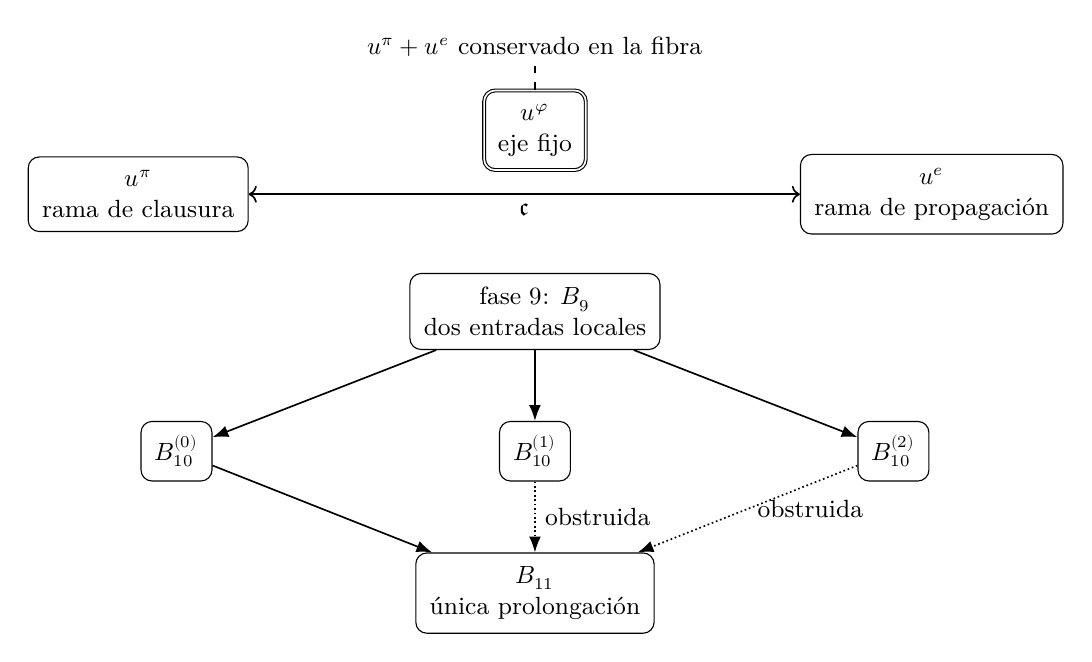
\begin{tikzpicture}[
 node distance=10mm and 15mm,
 every node/.style={font=\small,align=center},
 state/.style={draw=black,rounded corners,inner sep=5pt},
 inv/.style={draw=black,double,rounded corners,inner sep=5pt},
 arr/.style={-{Latex[length=2mm]},semithick}
]
 \node[state] (pi) {$u^\pi$\\rama de clausura};
 \node[state,right=70mm of pi] (e) {$u^e$\\rama de propagación};
 \coordinate (mirroraxis) at ($(pi)!0.5!(e)$);
 \node[inv,above=3mm of mirroraxis] (phi) {$u^\varphi$\\eje fijo};
 \draw[arr,<->] (pi) -- node[below] {$\mathfrak c$} (e);
 \node[above=3mm of phi] (aggregate)
   {$u^\pi+u^e$ conservado en la fibra};
 \draw[dashed] (phi.north) -- (aggregate.south);
 \node[state,below=10mm of mirroraxis] (b9) {fase $9$: $B_9$\\dos entradas locales};
 \node[state,below left=9mm and 25mm of b9] (b100) {$B_{10}^{(0)}$};
 \node[state,below=9mm of b9] (b101) {$B_{10}^{(1)}$};
 \node[state,below right=9mm and 25mm of b9] (b102) {$B_{10}^{(2)}$};
 \node[state,below=9mm of b101] (b11) {$B_{11}$\\única prolongación};
 \draw[arr] (b9) -- (b100);
 \draw[arr] (b9) -- (b101);
 \draw[arr] (b9) -- (b102);
 \draw[arr] (b100) -- (b11);
 \draw[arr,densely dotted] (b101) -- node[right] {obstruida} (b11);
\draw[arr,densely dotted] (b102) -- node[right] {obstruida} (b11);
\end{tikzpicture}
\end{document}
